 % !TeX document-id = {f19fb972-db1f-447e-9d78-531139c30778}
% !BIB program = biber

%\documentclass[handout]{beamer}
\documentclass[compress]{beamer}
\usepackage[T1]{fontenc}
\usetheme[block=fill,subsectionpage=progressbar,sectionpage=progressbar]{metropolis} 
\usepackage{graphicx}

\usepackage{wasysym}
\usepackage{etoolbox}
\usepackage[utf8]{inputenc}

\usepackage{threeparttable}
\usepackage{subcaption}

\usepackage{tikz-qtree}
\setbeamercovered{still covered={\opaqueness<1->{5}},again covered={\opaqueness<1->{100}}}


% color-coded listings; replace those above 
\usepackage{xcolor}
\usepackage{minted}
\definecolor{listingbg}{rgb}{0.87,0.93,1}
\setminted[python]{
	frame=none,
	framesep=1mm,
	baselinestretch=1,
	bgcolor=listingbg,
	fontsize=\scriptsize,
	linenos,
	breaklines
}



\usepackage{listings}

\lstset{
	basicstyle=\scriptsize\ttfamily,
	columns=flexible,
	breaklines=true,
	numbers=left,
	%stepsize=1,
	numberstyle=\tiny,
	backgroundcolor=\color[rgb]{0.85,0.90,1}
}


\lstnewenvironment{lstlistingoutput}{\lstset{basicstyle=\footnotesize\ttfamily,
		columns=flexible,
		breaklines=true,
		numbers=left,
		%stepsize=1,
		numberstyle=\tiny,
		backgroundcolor=\color[rgb]{.7,.7,.7}}}{}


\lstnewenvironment{lstlistingoutputtiny}{\lstset{basicstyle=\tiny\ttfamily,
		columns=flexible,
		breaklines=true,
		numbers=left,
		%stepsize=1,
		numberstyle=\tiny,
		backgroundcolor=\color[rgb]{.7,.7,.7}}}{}



\usepackage[american]{babel}
\usepackage{csquotes}
\usepackage[style=apa, backend = biber]{biblatex}
\DeclareLanguageMapping{american}{american-UoN}
\addbibresource{../../literature.bib}
\renewcommand*{\bibfont}{\tiny}

\usepackage{tikz}
\usetikzlibrary{shapes,arrows,matrix}
\usepackage{multicol}

\usepackage{subcaption}

\usepackage{booktabs}
\usepackage{graphicx}



\makeatletter
\setbeamertemplate{headline}{%
	\begin{beamercolorbox}[colsep=1.5pt]{upper separation line head}
	\end{beamercolorbox}
	\begin{beamercolorbox}{section in head/foot}
		\vskip2pt\insertnavigation{\paperwidth}\vskip2pt
	\end{beamercolorbox}%
	\begin{beamercolorbox}[colsep=1.5pt]{lower separation line head}
	\end{beamercolorbox}
}
\makeatother



\setbeamercolor{section in head/foot}{fg=normal text.bg, bg=structure.fg}



\newcommand{\question}[1]{
	\begin{frame}[plain]
		\begin{columns}
			\column{.3\textwidth}
			\makebox[\columnwidth]{
				
\includegraphics[width=\columnwidth,height=\paperheight,keepaspectratio]{../../pictures/mannetje.png}}
			\column{.7\textwidth}
			\large
			\textcolor{orange}{\textbf{\emph{#1}}}
		\end{columns}
\end{frame}}



\title[Big Data and Automated Content Analysis]{\textbf{A Practical Introduction to Machine Learning in Python} \\Day 2 - Tuesday Morning \\ »From text to features: Natural Language Processing«}
\author[Rupert Kiddle, Sjoerd Stolwijk]{Rupert Kiddle \\ Sjoerd Stolwijk \\ ~ \\ \footnotesize{r.t.kiddle@vu.nl, @rptkiddle \\ s.b.stolwijk@uu.nl} \\}
\date{September 16, 2025}
\institute[Gesis]{Gesis}\part{\part{title}}


\begin{document}
	
	\begin{frame}{}
		\titlepage{\tiny }
	\end{frame}
	
	\begin{frame}{Today}
		\tableofcontents
	\end{frame}


\section{Bottom-up vs. top-down}

\begin{frame}[standout]
Automated content analysis can be either \textcolor{red}{bottom-up} (inductive, explorative, pattern recognition, \ldots) or \textcolor{red}{top-down} (deductive, based on a-priori developed rules, \ldots). Or in between.
\end{frame}


\begin{frame}{The ACA toolbox}
\makebox[\columnwidth]{
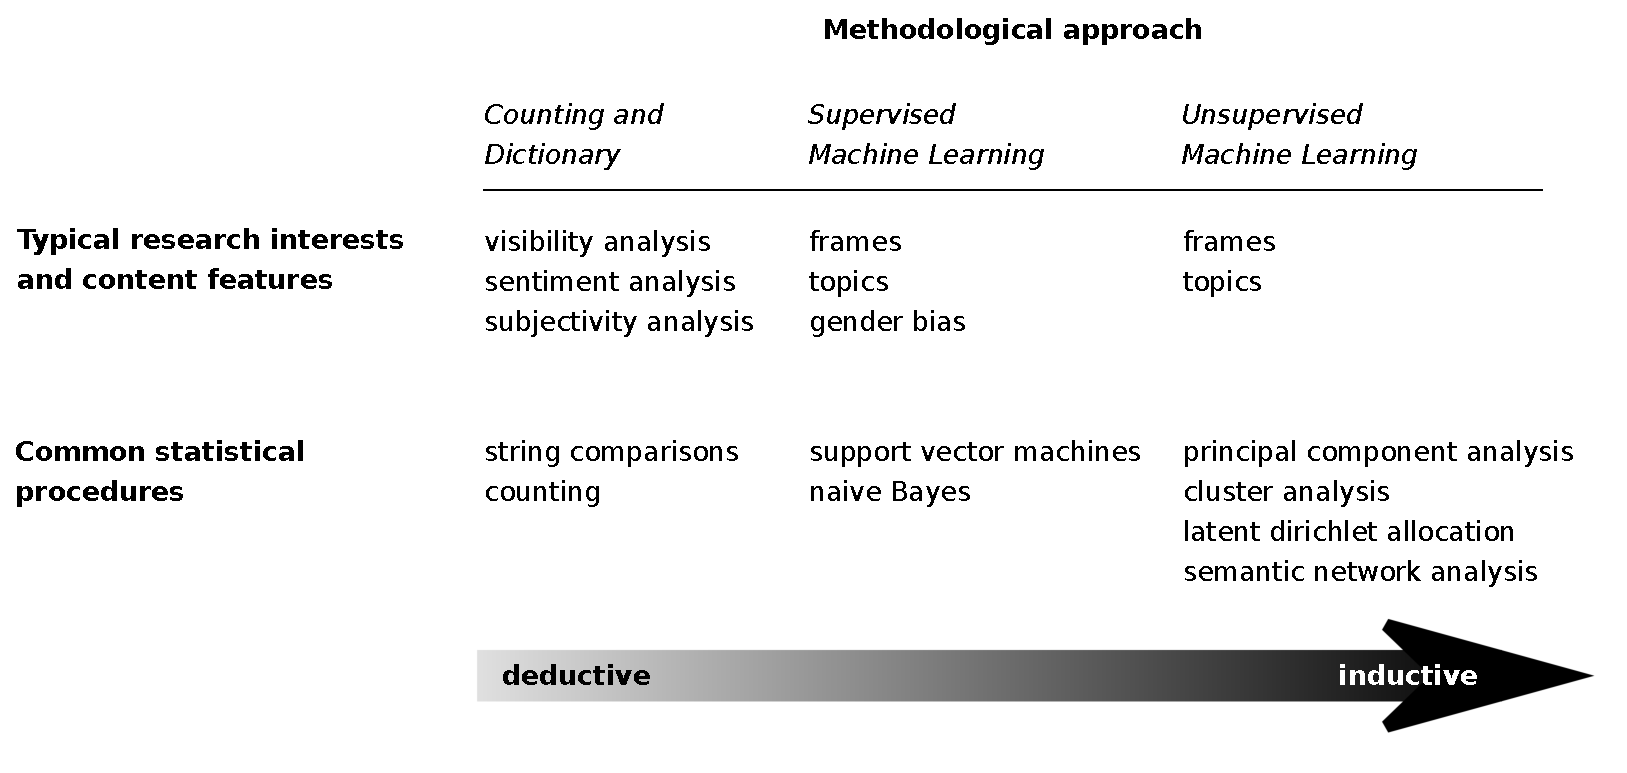
\includegraphics[width=\columnwidth,height=\paperheight,keepaspectratio]{../../pictures/boumanstrilling2016}}
\\
\cite{Boumans2016}
\end{frame}


\begin{frame}{Bottom-up vs. top-down}
\begin{block}{Bottom-up}
\begin{itemize}
\item Count most frequently occurring words 
\item Maybe better: Count combinations of words $\Rightarrow$ Which words co-occur together?
\end{itemize}
We \emph{don't} specify what to look for in advance	
\end{block}

\onslide<2>{
\begin{block}{Top-down}
\begin{itemize}
	\item Count frequencies of pre-defined words
	\item Maybe better: patterns instead of words
\end{itemize}
We \emph{do} specify what to look for in advance	
\end{block}
}
\end{frame}


\begin{frame}[fragile]{A simple bottom-up approach}
\begin{lstlisting}
from collections import Counter

texts = ["I really really really love him, I do", "I hate him"]

for t in texts:
    print(Counter(t.split()).most_common(3))
\end{lstlisting}
\begin{lstlistingoutput}
[('really', 3), ('I', 2), ('love', 1)]
[('I', 1), ('hate', 1), ('him', 1)]
\end{lstlistingoutput}
\end{frame}


\begin{frame}[fragile]{A simple top-down approach}
\begin{lstlisting}
texts = ["I really really really love him, I do", "I hate him"]
features = ['really', 'love', 'hate']

for t in texts:
    print(f"\nAnalyzing '{t}':")
    for f in features:
        print(f"{f} occurs {t.count(f)} times")
\end{lstlisting}
\begin{lstlistingoutput}
Analyzing 'I really really really love him, I do':
really occurs 3 times
love occurs 1 times
hate occurs 0 times

Analyzing 'I hate him':
really occurs 0 times
love occurs 0 times
hate occurs 1 times

\end{lstlistingoutput}
\end{frame}



\question{When would you use which approach?}


\begin{frame}{Some considerations}
\begin{itemize}[<+->]
	\item Both can have a place in your workflow (e.g., bottom-up as first exploratory step)
	\item You have a clear theoretical expectation? Bottom-up makes little sense.
	\item But in any case: you need to transform your text into something ``countable''.
\end{itemize}
\end{frame}


\section{Basic string operations}

\begin{frame}{Working with strings}
\begin{enumerate}[<+->]
\item string methods that every string has (\texttt{"hello".upper()})
\item functions that take a string as input (\texttt{len("hello")})
\item pandas column string methods (\texttt{df["somecolumn"].str.upper()})
\item applying string methods or functions to a pandas column (\texttt{df["somecolumn"].apply(len)} or \texttt{df["somecolumn"].apply(lambda x: x.upper()})
\end{enumerate}

\pause
For today, we assume that our data are a list of strings -- adapt accordingly for pandas.
\end{frame}


\begin{frame}[fragile]{An example says more than 1000 words\ldots}
\begin{minted}{python}
# probably read from text file(s) instead, you learned that already...
data = [ "I <b>really</b> liked this movie! It was great.  ", "  What an awful movie", "Awesome!!!"]

data_stripped = [e.strip() for e in data]
data_lower = [e.lower() for e in data_stripped]
data_clean = [e.replace("<b>",").replace("</b>",") for e in data_lower]

# or, more efficient, in one single step:
data_clean2 = [e.strip().lower().replace("<b>","").replace("</b>","") for e in data]
\end{minted}
\end{frame}



\begin{frame}[fragile]{Two examples says even more:}
\begin{minted}{python}
from string import punctuation

# punctuation is just the string '!"#$%&\'()*+,-./:;<=>?@[\\]^_`{|}~'

text = "This is a test! Let's get rid (of) punct&"

# we make a list of each character in the text but only if it is not
# a punctuation sign. The, we join the elements of the list directly
# to each other without anything between it ("")
cleantext = "".join([c for c in text if c not in punctuation])
\end{minted}
\end{frame}


\begin{frame}[fragile]{Combine both}
\begin{minted}{python}
from string import punctuation

def strip_punctuation(text):
    return "".join([c for c in text if c not in punctuation])

data_clean3 = [strip_punctuation(e).strip().lower()\
   .replace("<b>","").replace("</b>","") for e in data]
    
\end{minted}
\end{frame}




\begin{frame}{The toolbox at a glance}
  \footnotesize
\begin{block}{Slicing}
\texttt{mystring[2:5]} to get the characters with indices 2,3,4
\end{block}

\begin{block}{String methods}
\begin{itemize}
	\item \texttt{.lower()} returns lowercased string
	\item \texttt{.strip()} returns string without whitespace at beginning and end
	\item \texttt{.find("bla")} returns index of position of substring ``bla'' or -1 if not found
	\item \texttt{.replace("a","b")} returns string with "a" replaced by "b"
	\item \texttt{.count("bla")} counts how often substring ``bla'' occurs
        \item \texttt{.isdigit()} true if only numbers
          
\end{itemize}
Use tab completion for more!
\end{block}
\end{frame}




\begin{frame}[fragile]{From test to large-scale analysis: General approach}
1. Take a single string and test your idea
\begin{lstlisting}
t = "This is a test test test."
print(t.count("test"))
\end{lstlisting}
2a. You'd assume it to return 3. If so, scale it up:
\begin{lstlisting}
results = []
for t in listwithallmytexts:
    r = t.count("test")
    print(f"{t} contains the substring {r} times")
    results.append(r)
\end{lstlisting}

2b. If you \emph{only} need to get the list of results, a list comprehension is more elegant:
\begin{lstlisting}
results = [t.count("test") for t in listwithallmytexts]
\end{lstlisting}


\end{frame}


\begin{frame}[fragile]{General approach}
\Large

\textcolor{red}{Test on a single string, then make a for loop or list comprehension!}

\pause

\normalsize

\begin{alertblock}{Own functions}
If it gets more complex, you can write your own function and then use it in the list comprehension:
\begin{lstlisting}
def mycleanup(t):
   # do sth with string t here, create new string t2
   return t2
  
results = [mycleanup(t) for t in allmytexts]
\end{lstlisting}
\end{alertblock}
\end{frame}


\begin{frame}[fragile]{Pandas string methods as alternative}
If you select column with strings from a pandas dataframe, pandas offers a collection of string methods (via \texttt{.str.}) that largely mirror standard Python string methods:

\begin{lstlisting}
df['newcoloumnwithresults'] = df['columnwithtext'].str.count("bla")
\end{lstlisting} 


\pause

\begin{alertblock}{To pandas or not to pandas for text?}
Partly a matter of taste. 

Not-too-large dataset with a lot of extra columns? Advanced statistical analysis planned? Sounds like pandas.

It's mainly a lot of text? Wanna do some machine learning later on anyway? It's large and (potentially) messy? Doesn't sound like pandas is a good idea.
\end{alertblock}

\end{frame}





\subsection{A cleaner BOW representation}

\begin{frame}{Room for improvement}
\begin{description}
	\item[tokenization] How do we (best) split a sentence into tokens (terms, words)?
	\item[pruning] How can we remove unneccessary words?
	\item[lemmatization] How can we make sure that slight variations of the same word are not counted differently?

\end{description}
\end{frame}

\subsubsection{Better tokenization}

\begin{frame}[fragile]{OK, good enough, perfect?}
\begin{block}{.split()}
\begin{itemize}
	\item space $\rightarrow$ new word
	\item no further processing whatsoever
	\item thus, only works well if we do a preprocessing outselves (e.g., remove punctuation)
\end{itemize}
\end{block}
\begin{lstlisting}
docs = ["This is a text",  "I haven't seen John's derring-do. Second sentence!"]
tokens = [d.split() for d in docs]
\end{lstlisting}
\begin{lstlistingoutputtiny}
[['This', 'is', 'a', 'text'], ['I', "haven't", 'seen', "John's", 'derring-do.', 'Second', 'sentence!']]
\end{lstlistingoutputtiny}
\end{frame}


\begin{frame}{OK, good enough, perfect?}
  \begin{block}{Tokenizers from the NLTK pacakge}
    \begin{itemize}
    \item multiple improved tokenizers that can be used instead of .split()
    \item e.g., Treebank tokenizer:
      \begin{itemize}
      \item split standard contractions ("don't")
      \item deals with punctuation
      \item BUT: Assumes lists of \emph{sentences}.
      \end{itemize}
    \item Solution: Build an own (combined) tokenizer (next slide)!
    \end{itemize}
  \end{block}
\end{frame}


\begin{frame}[fragile]{OK, good enough, perfect?}
\begin{minted}{python}
import nltk
import regex

class MyTokenizer:
    def tokenize(self, text):
        tokenizer = nltk.tokenize.TreebankWordTokenizer()
        result = []
        word = r"\p{letter}"
        for sent in nltk.sent_tokenize(text):
            tokens = tokenizer.tokenize(sent)    
            tokens = [t for t in tokens 
                      if regex.search(word, t)]
            result += tokens
        return result
        
mytokenizer = MyTokenizer()
tokens = [mytokenizer.tokenize(d) for d in docs]

\end{minted}

\begin{lstlistingoutputtiny}
[['This', 'is', 'a', 'text'], ['I', 'have', "n't", 'seen', 'John', "'s", 'derring-do', 'Second', 'sentence']]
\end{lstlistingoutputtiny}
\end{frame}









\subsubsection{Stopword removal}



\begin{frame}{Stopword removal}
	\begin{block}{What are stopwords?}
		\begin{itemize}
			\item Very frequent words with little inherent meaning
			\item \texttt{the, a, he, she, \ldots}
			\item context-dependent: if you are interested in gender, \texttt{he} and \texttt{she} are no stopwords. 
			\item Many existing lists as basis
		\end{itemize}
	\end{block}

\end{frame}


\begin{frame}{Stopword removal: What and why?}
	\begin{block}{Why remove stopwords?}
		\begin{itemize}
			\item If we want to identify key terms (e.g., by means of a word count), we are not interested in them
			\item If we want to calculate document similarity, it might be inflated
			\item If we want to make a word co-occurance graph, irrelevant information will dominate the picture
		\end{itemize}
	\end{block}
\end{frame}

\begin{frame}[fragile]{Stopword removal}
	\begin{lstlisting}
from nltk.corpus import stopwords
mystopwords = stopwords.words("english")
mystopwords.extend(["test", "this"])
		
def tokenize_clean(s, stoplist):
    cleantokens = []
    for w in TreebankWordTokenizer().tokenize(s):
        if w.lower() not in stoplist:
            cleantokens.append(w)
	return cleantokens
		
tokens = [tokenize_clean(d, mystopwords) for d in docs]
	\end{lstlisting}
	\begin{lstlistingoutputtiny}
[['text'], ["n't", 'seen', 'John', 'derring-do.', 'Second', 'sentence', '!']]
	\end{lstlistingoutputtiny}

\begin{alertblock}{You can do more!}
	\tiny{For instance, in line 8, you could add an \texttt{or} statement to also exclude punctuation.}
\end{alertblock}

\end{frame}

\begin{frame}[fragile]{Removing punctuation}
	\begin{lstlisting}
from nltk.tokenize import RegexpTokenizer
tokenizer = RegexpTokenizer(r'\w+')
tokenizer.tokenize("Hi all, what's up!")
	\end{lstlisting}  
	\begin{lstlistingoutputtiny}
['Hi', 'all', 'what', 's', 'up']
	\end{lstlistingoutputtiny}
	\begin{lstlisting}
from string import punctuation
doc = "She said, of course i'll come to the party!!!"
"".join([w for w in doc if w not in punctuation])
\end{lstlisting}  
	\begin{lstlistingoutputtiny}
'She said of course ill come to the party'
	\end{lstlistingoutputtiny}
	
\end{frame}

\subsection{Stemming and lemmatization}


\begin{frame}{NLP: What and why?}
	\begin{block}{Why do stemming?}
		\begin{itemize}
			\item Because we do not want to distinguish between smoke, smoked, smoking, \ldots
			\item Typical preprocessing step (like stopword removal)
		\end{itemize}
	\end{block}
\end{frame}

\begin{frame}[fragile]{Stemming and lemmatization}
	\begin{itemize}
		\item Stemming: reduce words to its stem by removing last part (drinking $\rightarrow$ drink)
		\item Lemmatization: find word that you would need to look up in a dictionary (drinking $\rightarrow$ drink, but also went $\rightarrow$ go)
		\item stemming is simpler than lemmatization
		\item lemmatization often better
	\end{itemize}
	\pause
	
	Example below: tokenization and lemmatization with \texttt{spacy} in one go:
	\begin{lstlisting}
		import spacy
		nlp = spacy.load('en')   # potentially you need to install the language model first
		lemmatized_tokens = [[token.lemma_  for token in nlp(doc)] for doc in docs]
	\end{lstlisting}
	\begin{lstlistingoutputtiny}
		[['this', 'be', 'a', 'text'], ['-PRON-', 'have', 'not', 'see', 'John', "'s", 'derring', '-', 'do', '.', 'second', 'sentence', '!']]
	\end{lstlistingoutputtiny}
\end{frame}




\begin{frame}[fragile]{Stemming and stopword removal - let's combine them!}
	\begin{lstlisting}
from nltk.stem.snowball import SnowballStemmer
from nltk.corpus import stopwords
stemmer=SnowballStemmer("english")
mystopwords = stopwords.words("english")
frase="I am running while generously greeting my neighbors"
frasenuevo=""
for palabra in frase.lower().split():
	if palabra not in mystopwords:
	frasenuevo=frasenuevo + stemmer.stem(palabra)  + " "
\end{lstlisting}
Now, {\tt{print(frasenuevo)}} returns:
\begin{lstlisting}
run generous greet neighbor
	\end{lstlisting}
	Perfect!
	\pause
	\small
	Or:
	\begin{lstlisting}
print(" ".join([stemmer.stem(p) for p in frase.lower().split() if p not in mystopwords]))
	\end{lstlisting}
	
\end{frame}

\subsection{ngrams}
\begin{frame}
	Instead of just looking at single words (unigrams), we can also use adjacent words (bigrams).
\end{frame}

\begin{frame}[fragile]{ngrams}
	\begin{lstlisting}
import nltk
texts = ['This is the first text text text first', 'And another text yeah yeah']
texts_bigrams = [["_".join(tup) for tup in nltk.ngrams(t.split(),2)] for t in texts]
print(texts_bigrams)
	\end{lstlisting}
	\texttt{[['This\_is',
		'is\_the',
		'the\_first',
		'first\_text',
		'text\_text',
		'text\_text',
		'text\_first'],
		['And\_another', 'another\_text', 'text\_yeah', 'yeah\_yeah']]
	}
	
	Typically, we would combine both.
	\pause
	\textbf{\textcolor{red}{What do you think? Why is this useful? (and what may be drawbacks?)}}
\end{frame}



\subsection{The order of preprocessing steps}

\begin{frame}{Option 1}
\begin{block}{Preprocessing only through Vectorizer}
``Just use CountVectorizer or Tfidfvectorizer with the appropriate options.''	
\begin{itemize}
	\item pro: No double work, efficient if your main goal is a sparse matrix (for ML?) anyway
	\item con: you cannot ``see'' the preprocessed texts
\end{itemize}
\end{block}
\end{frame}

\begin{frame}[fragile]{Option 2}
	\begin{block}{Extensive preprocessing without Vectorizer}
``Remove stopwords, punctuation etc. and store in a string with spaces''

\begin{lstlisting}
cleaneddocs = [" ".join(re.findall(r"\w\w+", d)).lower() for d in docs]
cleaneddocswithoutstopwords = [" ".join([w for w in d.split() if w not in mystopwords]) for d in cleaneddocs]
\end{lstlisting}
\begin{lstlistingoutputtiny}
['this is text', 'haven seen john derring do second sentence']
['text', 'seen john derring second sentence']	
\end{lstlistingoutputtiny}
{\tiny{Yes, this list comprehension looks scary -- you can make a more elaborate for loop instead}}
	
\begin{itemize}
	\item pro: you can read (and store!) the preprocessed docs
	\item pro: even the most stupid vectorizer (or wordcloud tool) can split the resulting string later on
	\item con: potentially double work (for you \emph{and} the computer)
\end{itemize}
\end{block}
\end{frame}


\question{How would you do it?}

\begin{frame}[plain]
Sometimes, I go for Option 2 because
\begin{itemize}
	\item I like to inspect a sample of the documents
	\item I can re-use the cleaned docs irrespective of the Vectorizer
\end{itemize}

But at other times, I opt of Option 1 instead because
\begin{itemize}
	\item I want to systematically compare the effect of different choices in a machine learning pipeline (then I can simply vary the vectorizer instead of the data)
	\item I want to use techniques that are geared towards little or no preprocessing (deep learning)
\end{itemize}

\end{frame}


\subsection{How further?}


\begin{frame}{Main takeaway}

\begin{itemize}
	\item It matters how you transform your text into numbers (``vectorization'').
	\item Preprocessing matters, be able to make informed choices.
	\item Keep this in mind when we will discuss Machine Learning! It will come back throughout Part II!
\end{itemize}

\begin{itemize}
	\item Once you vectorized your texts, you can do all kinds of calculations (random example: get the cosine similarity between two texts)
\end{itemize}

\end{frame}


\begin{frame}{More NLP}
\begin{description}
	\item[$n$-grams] Consider using $n$-grams instead of unigrams
	\item[collocations]  $n$grams that appear more frequently than expected
	\item[POS-tagging] grammatical function (``part-of-speach'') of tokens
	\item[NER] named entity recognition (persons, organizations, locations)
\end{description}
\end{frame}

\begin{frame}{More NLP}
I \textbf{really} recommend looking into spacy (\url{https://spacy.io}) for advanced natural language processing, such as part-of-speech-tagging and named entity recogntion.
\end{frame}





\begin{frame}[fragile]{General approach}
\Large

\textcolor{red}{Test on a single string, then make a for loop or list comprehension!}

\pause

\normalsize

\begin{alertblock}{Own functions}
If it gets more complex, you can write your ow= function and then use it in the list comprehension:
\begin{lstlisting}
def mycleanup(t):
    # do sth with string t here, create new string t2
    return t2

results = [mycleanup(t) for t in allmytexts]
\end{lstlisting}
\end{alertblock}
\end{frame}


\begin{frame}[fragile]{Pandas string methods as alternative}
If you select column with strings from a pandas dataframe, pandas offers a collection of string methods (via \texttt{.str.}) that largely mirror standard Python string methods:

\begin{lstlisting}
df['newcoloumnwithresults'] = df['columnwithtext'].str.count("bla")
\end{lstlisting} 


\pause

\begin{alertblock}{To pandas or not to pandas for text?}
Partly a matter of taste. 

Not-too-large dataset with a lot of extra columns? Advanced statistical analysis planned? Sounds like pandas.

It's mainly a lot of text? Wanna do some machine learning later on anyway? It's large and (potentially) messy? Doesn't sound like pandas is a good idea.
\end{alertblock}

\end{frame}



%\begin{frame}[plain]
%	\printbibliography
%\end{frame}



\end{document}



